\documentclass[pdftex]{article}
\usepackage[T1]{fontenc}
\usepackage[utf8]{inputenc}
\usepackage{graphicx}
\usepackage{caption}

\title{PHYS 721 Homework 2}
\author{Nick Tyler}
\date{}


\begin{document}
\maketitle
\begin{enumerate}
	\item The values the first column in data set were plotted as a histogram
	to represent the energy of the particle. \\
	\parbox{\linewidth}{\centering
		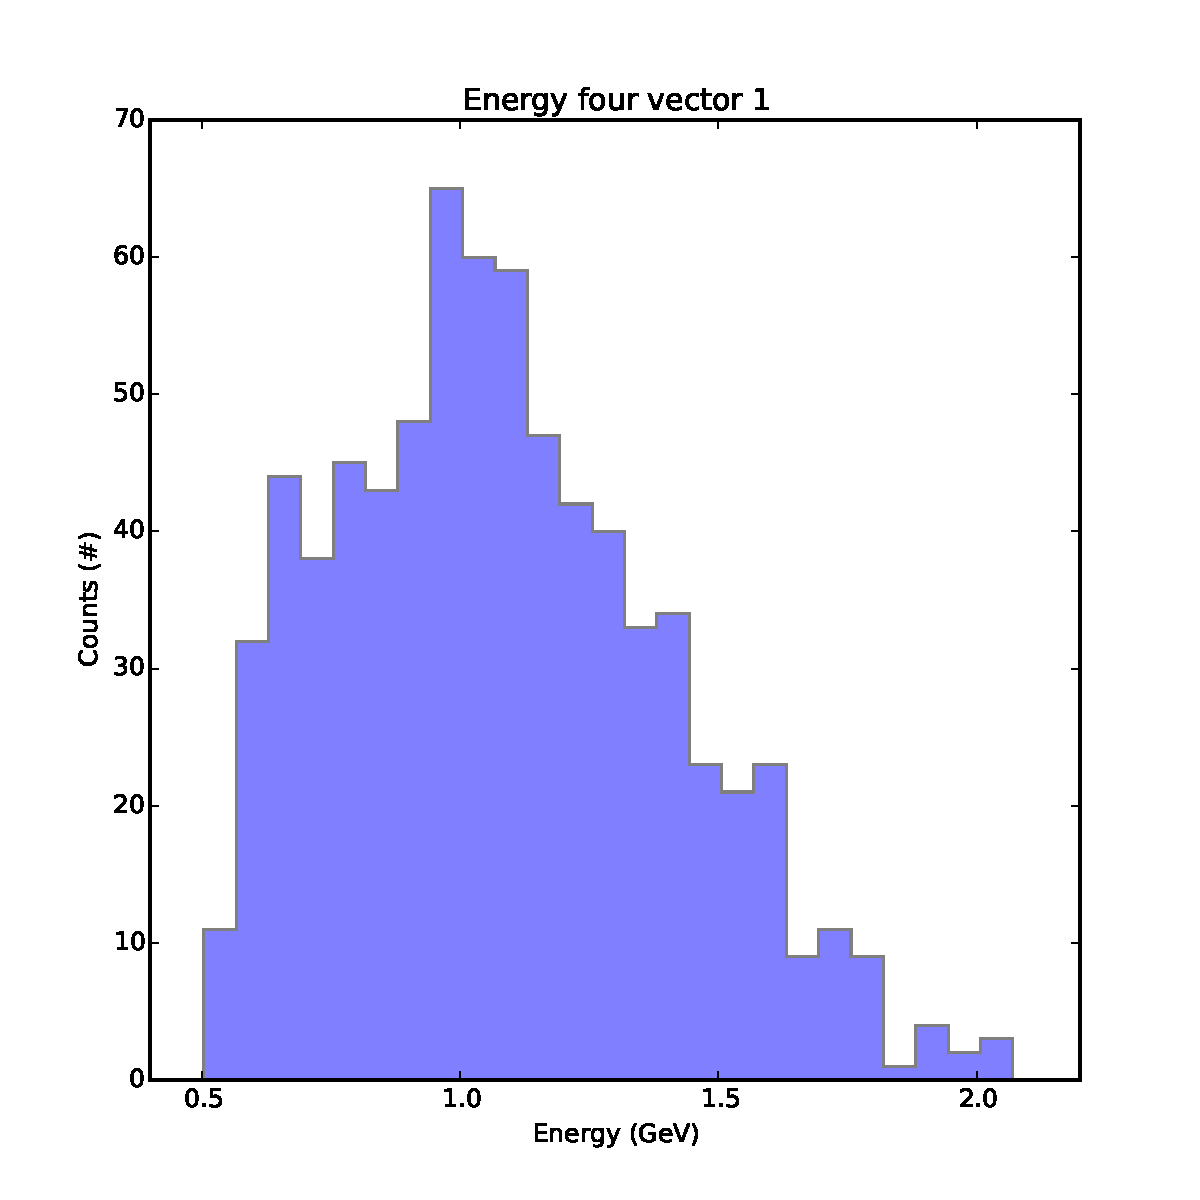
\includegraphics[scale=0.5]{Problem_1.pdf}\\
		\captionof{figure}{Energy Histogram in GeV}
	}
	\newpage
	\item The mass of the four vectors was calculated by finding the magnitude of the four vector 
	($m = \sqrt{E^2 - P_x^2 - P_y^2 - P_z^2}$).
	Using ROOT's TLorentzVector class this can easily be done by filling the four vectors and 
	using the built in magnitude function.  The third histogram represents the mass of the sum
	of the compenemts of the two four vectors.\\
	\parbox{\linewidth}{\centering
		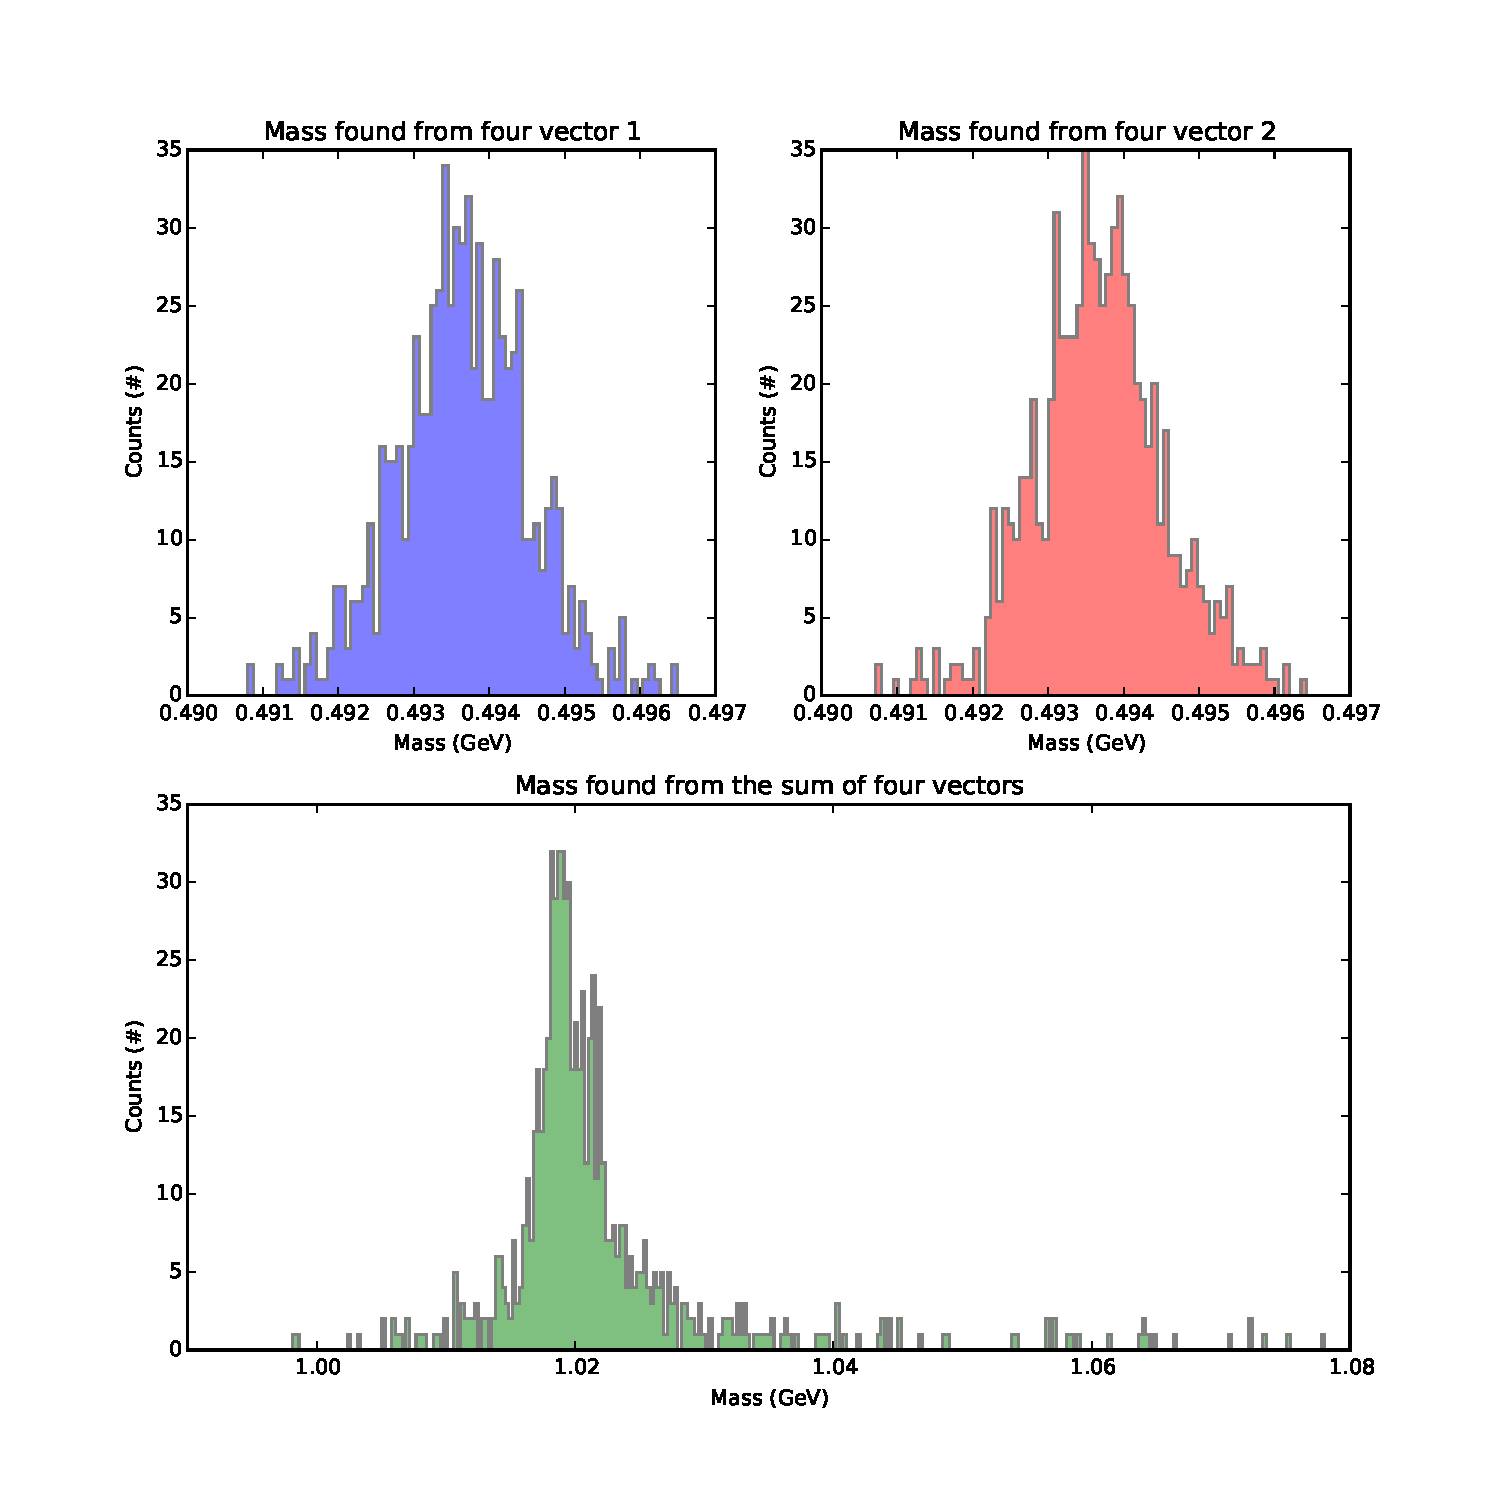
\includegraphics[scale=0.5]{Problem_2.pdf}\\
		\captionof{figure}{Mass Histograms in GeV/$c^2$}
	}

\end{enumerate}

\end{document}